\documentclass[course=erap]{aspdoc}

\usepackage{pgfplots}
\usepackage{tikz}
\usepackage{hyperref}

\newcommand{\theGroup}{134}
\newcommand{\theNumber}{A404}
\author{Arman Habibi \and Larissa Manalil \and Andrei Stoica}
\date{Wintersemester 2022/23}

\title{Gruppe \theGroup{} -- Abgabe zu Aufgabe \theNumber}

\begin{document}
\maketitle

\section{Einleitung}
\subsection{Überblick}

Wir befinden uns seit einigen Jahrzehnten in der Ära der Big Data. Schnell wachsende und komplexe Datenmengen treffen auf herkömmliche Verarbeitungsmethoden, welche diese nicht oder nur schwer verarbeiten können. Daher spielt Datenkompression in der heutigen Zeit eine große Rolle.\\
Viele Computer benutzen die Extended-ASCII-Kodierung, um Buchstaben digital darzustellen. Dabei steht ASCII für \textit{American Standard Code for Information Interchange}, welches 256 Symbole mit genau acht Bits repräsentieren kann.\cite{Ascii} Beachtet man jedoch, dass Symbole in einem Text unterschiedlich oft auftauchen, könnte man Zeichen, die öfters vorkommen, mit weniger Bits kodieren als Zeichen, die seltener vorkommen. Dadurch wird der Text zum Schluss platzsparender gespeichert.\\
Dies ist das grundlegende Konzept der im Jahr 1952 von \textit{David A. Huffman} entwickelten Huffman-Kodierung mit dem Ziel, eine einfache und verlustfreie Datenkompression zu ermöglichen.
\subsection{Konzept}
Dabei werden nach einer Häufigkeitsanalyse der Symbole im gegebenen Text diese in einem binären Huffman-Baum angeordnet, welcher jedem Zeichen eine entsprechende Bitsequenz zuordnet. Die Besonderheit des Huffman-Baums liegt darin, dass die Symbole nur in den Blättern des Baumes gespeichert werden, wodurch präfix-freie Sequenzen geschafft werden. Damit wird eine Unverwechselbarkeit garantiert, woraus folgt, dass keine Bitfolge mit dem Anfang einer anderen übereinstimmt. Sobald bei der Kodierung ein Zeichen zugeordnet worden ist, beginnt direkt die Bitfolge des nächsten Symbols. Dies ermöglicht es, die Daten ohne Trennzeichen zu speichern, und somit Redundanz zu minimieren.\\
Im Folgenden wird als Beispiel der String \textit{ANANASSAFT} komprimiert, welcher aus folgenden Häufigkeiten hervorgeht. Hierbei wurden nicht vorhandene Zeichen vernachlässigt.\\
\begin{center}
    \begin{tabular}{ c|c|c|c|c|c } 
     \textbf{Zeichen} & A & F & N & S & T \\ 
     \hline
     \textbf{Häufigkeit} & 4 & 1 & 2 & 2 & 1 \\
    \end{tabular}
\end{center}
Daraufhin wird der präfix-freie Huffman-Baum erstellt, welcher jedem Symbol ihre Bitsequenzen zuordnet. Die Zuordnung einer Bitfolge zu einem Symbol erfolgt durch das Traversieren %(?) 
des Baumes von der Wurzel bis zum jeweiligen Zeichen. Muss man dabei ein Knoten nach links beziehungsweise rechts, wird eine 0 beziehungsweise 1 an die kodierte Bitfolge drangehängt.
\begin{center}
    \begin{tikzpicture}
            \node{10} [sibling distance = 2cm, level distance = 0.7cm]
            child {node {A:4} }
            child {node {6} child {node {N:2}}
            child {node {4} child {node {S:2}}
            child {node {2} child {node {F:1}} child {node {T:1}}}}};
    \end{tikzpicture}
    \\Abb. 1: Konstruierter Huffmanbaum
    \label{fig:my_label}
\end{center}
Mit der folgenden Zuweisung der Symbole kann das Beispiel nun dekodiert werden. Die Gruppierung der Bits dient nur dem visuellen Verständnis.
\begin{center}
    \begin{tabular}{c|c}
        \textbf{Symbol} & \textbf{Bitsequenz} \\
        \hline
        A & 0 \\
        F & 1110 \\
        N & 10 \\
        S & 110 \\
        T & 1111
    \end{tabular}
    \label{tab:my_label}
\end{center}
\begin{center}
    ANANASSAFT = 0 10 0 10 0 110 110 0 1110 1111
\end{center}
Ursprünglich hätte das Beispiel mit $10\cdot8 = 80$ Bits gespeichert werden müssen. Die Huffman-Kodierung reduziert das Wort auf insgesamt $1+2+1+2+1+3+3+1+4+4=22$ Bits. Jedoch muss zusätzlich auch der Huffmanbaum als Datenstruktur abgespeichert werden. Nichtsdestotrotz ermöglicht die Huffman-Kodierung bei vor allem längeren Texten ein geeignetes, platzsparendes Format zur Datenkompression, insofern die Häufigkeiten der Symbole bekannt sind. Auf das Format zum Speichern des Baumes wird später genauer eingegangen.\cite{4051119}\\
Im Folgenden wird eine Implementierung der Huffman-Kodierung in der Programmiersprache C vorgestellt, welche es ermöglicht, Eingabetext im Extended-ASCII Format zu (de-)kodieren. Im Anschluss dieser wird die Korrektheit der Implementierung analysiert. Zuletzt wurde die Performanz auf Kompressionsrate und Zeitmessungen untersucht, indem der Algorithmus mit einer nicht optimierten und einer Vergleichsimplementierung inspiziert wurde.

\section{Lösungsansatz}

Der Lösungsansatz beruht auf dem Einlesen eines maximal 65536 Zeichen langen Textes durch das C-Rahmenprogramm, welches an das Huffman Programm zum Komprimieren weitergegeben wird. Das Ergebnis, zusammengesetzt in einem speziellen Format, wird in die vom Nutzer spezifizierte Ausgabedatei geschrieben. Gleichermaßen funktioniert auch das Dekodieren komprimierter Dateien, jedoch müssen die Daten formatiert vorliegen, auf das später im Abschnitt \ref{sec:encode} genauer eingegangen wird.

\subsection{main.c}
In diesem Teil befindet sich das Rahmenprogramm. Die folgenden Argumente können mittels der Funktion \textit{getopt()} ausgelesen und die zugehörigen Flags gesetzt werden.\\
Ein Pfad zur Eingabedatei ist immer obligatorisch. Neben dieser gibt \textit{-V} an, welche Implementierung verwendet wird, \textit{-B} ob die Performanz gemessen werden soll und \textit{-o} bezeichnet den Name der Ausgabedatei. \textit{-d} entscheidet über die En-/Dekodierung. Falls das Argument \textit{-h} oder invalide Argumente gefunden werden, wird eine Hilfsnachricht ausgedruckt und das Programm mit einem entsprechenden Rückgabewert abgebrochen.\\
Anschließend wird die Eingabedatei und dessen Länge ausgelesen und gespeichert. Nun wird je nach gesetztem \textit{-d} Flag entweder die \textit{encode()} oder \textit{decode()} Funktion, mit dem String und dessen Länge als Parameter, aufgerufen.
Zum Schluss wird das Ergebnis des Huffman-Algorithmus wieder zurück in die Ausgabedatei geschrieben.

\subsection{tree.c/heap.c}
Um den oben genannten Baum generieren zu können, muss eine geeignete und effiziente Datenstruktur verwendet werden. Wir haben uns für eine Prioritätswarteschlange entschieden, welche Baumknoten beinhalten kann.\\
Ein Baum in C besteht üblicherweise aus einem Datensatz (hier: Buchstaben und Häufigkeit) und zwei Zeigern, welche auf die jeweiligen Kinder zeigen. In diesen werden zunächst nur einzelne Symbole und dessen Häufigkeit ohne Kinder gespeichert. Im Verlauf der Enkodierung wird hier schrittweise der Huffman-Baum generiert. Um in effizienter Zeit auf die kleinsten Häufigkeiten zugreifen zu können, bietet sich eine Prioritätswarteschlange an, welche als Min-Heap implementiert wurde.\\
In dieser gibt es ein Array bestehend aus Zeigern auf Knoten. Da ein Min-Heap auch wiederum als Baum implementiert ist, wird eine Referenzierung auf die Eltern-/Kindknoten mittels Indexierung durchgeführt. Um die Min-Heap Eigenschaft zu gewährleisten, wird nach einfügen (\textit{insert}) und herausnehmen (\textit{pop\textunderscore min}) von Elementen \textit{heapified}. Dies bedeutet, dass je nach Kontext von oben oder von unten heraus so lange rekursiv Knoten getauscht werden, bis die Frequenz aller Elternknoten kleiner als die ihrer Kinder sind. Diese In-place Variante ermöglicht nicht nur eine sehr effiziente Zugriffszeit auf den Heap, sondern auch eine maximal logarithmische Laufzeit bei jeder Interaktion.

\subsection{huffman.c}
\subsubsection{encode}
\label{sec:encode}

Die Hauptfuntionalität, um Daten zu komprimieren, liegt in der folgenden Funktion:

\begin{center}
    \begin{lstlisting}[frame=single, framerule=0pt, numbers=none]
        char *huffman_encode(size_t len, const char data[len])
    \end{lstlisting}
\end{center}
Da die komprimierten Daten wieder in eine Datei geschrieben werden, wurde der Rückgabeparameter der Funktionssignatur von \textit{void} auf einen \textit{char}-Zeiger geändert.\\
Zuerst wird die Häufigkeitsanalyse der Symbole durchgeführt. Zunächst bestand die Idee, ein doppeltes Array zu allozieren, um im ersten Array alle Zeichen und im zweiten die entsprechenden Häufigkeiten zu speichern. Jedoch haben wir uns entschieden, eine speicherplatzeffizientere Methode zu nutzen.\\
Bei dieser wird eine Häufigkeitstabelle mit einer Größe von \textit{256} \textit{uint16\textunderscore t} Variablen alloziert und mit \textit{0} initialisiert. Da sich diese Huffman-Kodierung auf Kompression von Daten mit Zeichen der erweiterten ASCII Kodierung bezieht, repräsentiert jeder Index des Arrays das entsprechende ASCII-Zeichen. Da die \textit{BUF\textunderscore LENGTH} \textit{65535} beträgt, sind \textit{uint16\textunderscore t} Variablen für die Häufigkeit ausreichend.
Es wird durch die gesamte Datei iteriert, welches eine Laufzeit von $\mathcal{O}(n)$ beträgt, doch das Zählen erfolgt hierbei mit einer Effizienz von $\mathcal{O}(1)$, da der Array-Index dem ASCII-Code entspricht.
Anschließend wird der Huffmanbaum konstruiert, wobei eine Prioritätswarteschlange erstellt wird, welche ein Array mit Zeigern auf Knoten für jedes der \textit{256} ASCII Zeichen angelegt. Dies addiert sich auf etwa \textit{64 Bit $\cdot$ 256 = 2KiB}. Um Speicher zu sparen, werden Knoten, bestehend aus einem Symbol und deren Häufigkeit, erst erstellt und im Anschluss in den Heap eingefügt, sobald das zugehörige ASCII Zeichen nach der Häufigkeitstabelle schon gelesen wurde.\\
Solange mehr als ein Knoten im Min-Heap ist, werden die beiden Knoten mit der geringsten Frequenz aus dem Min-Heap entfernt und als Kindknoten an einem neuen Knoten (mit einem \textbackslash 0 Zeichen als Buchstaben) angehangen. Als Frequenz enthält dieser die Summe der beiden Kindfrequenzen. Dieser wird wieder in den Min-Heap eingefügt.
Übrig bleibt ein einzelner Knoten mit der den gesamten Huffman-Baum beinhaltet.\\
Im Anschluss wird der Ausgabestring generiert.\\
Neben den komprimierten Daten muss zusätzlich der Baum gespeichert werden, um den Text später dekodieren zu können. Um vom Vorteil der Huffman-Kodierung zu profitieren, muss ein insbesondere platzsparendes Format genutzt werden. Die Häufigkeit der einzelnen Zeichen ist für das Dekodieren irrelevant und wird daher nicht mitgespeichert.
Man traversiert, von der Wurzel aus gesehen, den Baum in Pre-Order Reihenfolge. Falls der jetzige Knoten ein Blatt ist, wird zuerst eine \textit{1} und anschließend die \textit{8} Bits für das ASCII-Symbol, welches das Blatt repräsentiert, in den Buffer geschrieben. Mithilfe von Bitmasken und Shifts wird laufzeiteffizient die \textit{8}-Bit-Folge des Zeichens generiert und gespeichert. Handelt es sich um kein Blattknoten, wird ein \textit{0}-Bit gespeichert. Daraufhin werden die beiden Kinder-Knoten kodiert, wobei erst das linke und dann das rechte betrachtet wird.
Für den Baum in Abbildung 1 würde die Baumkompression wie folgt aussehen:
\begin{center}
    01 01000001(A) 01 01001110(N) 01 01010011(S) 01 01000110(F) 1 01010100(T)
\end{center}
Beim Ausgabeformat haben wir uns dazu entschieden, den Baum genauso darzustellen, wie er im Speicher mit Bits gespeichert werden würde. Folglich haben wir auf die Buchstaben und Leerzeichen im Beispiel verzichtet. Nach der Baum-Bitfolge im Ausgabeformat wird ein Zeilenumbruch angehängt, worauf dann die kodierte Bitsequenz der Quelldatei folgt. Die Ausgabe ist dadurch nicht das am effizient möglichste Format, sollte jedoch eine gute Mitte zwischen einem menschenlesbarer und visuellansprechender Übersetzung bieten.\\
Für das eigentliche Kodieren der Eingabe wird mithilfe der Methode \textit{tree\textunderscore to\textunderscore dic(Node *root, uint8\textunderscore t *length\textunderscore table, uint32\textunderscore t *lookup\textunderscore table, uint32\textunderscore t path, uint8\textunderscore t length)} zunächst der Baum in ein Wörterbuch umgewandelt. Dabei wird im \textit{lookup}-Feld die kodierte Huffmanfolge für jedes Zeichen gespeichert und im \textit{length}-Feld die Länge der Sequenz. Auch hier wird rekursiv \textit{in-oder} Reihenfolge der Baum traversiert. Die Variable \textit{path} beschreibt den aktuellen Huffmancode des Durchlaufes und \textit{length} die aktuelle Länge. Als Beispiel wird bei einem rechten Durchlauf der Pfad erst um eins nach links geshiftet und anschließend mit \textit{1} verodert, um das Anfügen einer \textit{1} zu simulieren. Wenn ein valider Buchstabe gefunden wird, werden die beiden Variablen entsprechend in die Tabelle gesetzt.\\
Der Baum wird danach nicht mehr genutzt und daher freigegeben.\\
Zum Schluss werden die Zeichen der Eingabedatei mit Hilfe der zwei Felder komprimiert und an den Ausgabestring angehängt. Dabei wird eine for-Schleife der entsprechenden Größe genutzt, um unerlaubten Speicherzugriff zu vermeiden. Mithilfe von Bitmasken und Shifts wird effizient jedes Zeichen in ihre Huffman-Folge umgewandelt und an den Ausgabestring angehängt. Letztendlich wird dieser zurückgegeben.

\subsubsection{decode}
Das Dekodieren komprimierter Eingaben geschieht mit der folgenden Funktion:
\begin{center}
    \begin{lstlisting}[frame=single, framerule=0pt, numbers=none]
        char *huffman_decode(size_t len, const char data[len])
    \end{lstlisting}
\end{center}
Auch hier wird das Ergebnis in eine Datei geschrieben, weshalb der Rückgabeparameter der Funktionssignatur von \textit{void} auf ein \textit{char}-Zeiger verbessert wurde. Nach dem Allozieren von \textit{65536} Bytes an Speicher, wird nach einem Zeilenumbruch in der zu dekodierenden Eingabe gesucht, welches den Huffman-Baum von den komprimierten Code trennt. Falls bei der Iteration der Eingabe kein \textit{\textbackslash n} oder andere Zeichen außer \textit{0} und \textit{1} im Code gefunden werden, wird eine passende Fehlermeldung geworfen und \textit{NULL} zurückgegeben.\\
Daraufhin wird der Baum rekursiv gebildet. Man geht sequenziell durch die Bitsequenz, welche den Baum repräsentiert. Bei einem \textit{0}-Bit erstellt man einen \textit{NULL}-Knoten und ruft die Methode rekursive auf seinen linken und dann rechten Kindknoten auf. Bei einem \textit{1}-Bit erstellt man einen Blattknoten, der das ASCII-Zeichen beinhaltet. Nach einer \textit{1} folgen immer die \textit{8} Bits, die das ASCII-Zeichen als Bitsequenz identifizieren.\\
Letztendlich wird die komprimierte Datei dekodiert, indem diese iteriert und sequenziell abgearbeitet wird, um unerlaubten Speicherzugriff zu vermeiden.\\
Ein Zeiger fängt bei der Wurzel des Huffman-Baums an und geht bei einer \textit{0} beziehungsweise \textit{1} in der Bitsequenz zum linken beziehungsweise rechten Kindknoten. Falls es sich um einen Blattknoten handelt, wird das entsprechende Symbol in den Buffer geschrieben und man beginnt wieder an der Wurzel. Garantiert wird dieses Phänomen durch die bereits angesprochene Präfixfreiheit.\\
Zeigt der Zeiger zum Schluss nicht auf die Wurzel des Baums, wird eine Exception ausgegeben, da es sich um eine fehlerhafte Eingabe handelt.
Letztendlich werden alle Zeiger befreit und der Buffer zurückgegeben.

\section{Korrektheit}
Es wird auf die Korrektheit des Huffman Algorithmus eingegangen, da er verlustfreie Komprimierung ermöglicht und somit Genauigkeit als Begriff unangemessen wäre.
Um das Problem des optimalen und präfixfreien Codes zu lösen, sind zunächst einige Definitionen notwendig.

\subsection{Kodierungstheorie}

Das \textit{Quellalphabet} der Länge $n$ entspricht der Anzahl an verschiedenen Zeichen, die in der Quelldatei vorkommen. In diesem Fall entspricht das maximale Quellalphabet der Menge an ASCII Zeichen.
Jedem Zeichen wird ein \textit{Gewicht} $w$ zugeordnet, welches hier der absoluten Häufigkeit des Zeichens in der Quelldatei entspricht. Die Menge der Gewichte ist somit definiert als $W = \langle w_i > 0 \mid 0 \le i < n \rangle $.
Des Weiteren wird auch ein \textit{Codealphabet} definiert, welches die Binäre Menge $\lbrace0, 1\rbrace$ ist, mit dem die Quelldatei komprimiert wird.
Der \textit{Code} ordnet jedem Zeichen $i$ des Quellalphabets ein Codewort aus dem Codealphabet der Länge $l_i$ zu und ist definiert als die Menge $T = \langle l_i > 0 \mid 0 \le i < n \rangle$.\\
Die Kraft-McMillan-Ungleichung gilt als notwendige Bedingung für präfixfreie Codes.
$$\mathcal{K}(T) = \sum_{i=0}^{n-1} 2^{-l_i} \le 1$$
Codes, die diese Bedingung erfüllen, werden \textit{zulässig} genannt. Dies bedeutet, dass eine Belegung an Codewörten existiert, die präfixfrei sind.
Eine Menge an Codewörten ist für einen gegebenen Code \textit{gültig}, insofern die Längen $\langle l_i \rangle$ übereinstimmen und kein Codewort Präfix eines anderen ist.
Es ist somit möglich zu sagen, dass eine präfixfreier Code determiniert wurde, sobald ein zulässiger Code gefunden wurde, ohne die spezifischen Codewörter zu betrachten, da man weiß, dass eine gültige Belegung existiert.\\
Zuletzt sind noch die \textit{Kosten} $C$ eines Codes zu definieren, welches der Länge der kodierten Nachricht entspricht.
$$C(W,T) = C(\langle w_i \rangle,\langle l_i \rangle) = \sum_{i=0}^{n-1} w_i \cdot l_i $$
Ein Code $T = \langle l_i > 0 \mid 0 \le i < n \rangle$ gilt als optimal, falls für jeden anderen zulässigen Code T' der Länge $n$ gilt: $C(W,T) \le C(W,T^{\prime})$. Dies bedeutet auch, dass mehrere optimale Codes für eine gegebene Quelldatei existieren können.
Für einen optimalen Code muss die Kraft-McMillan-Summe 1 ergeben, da bei kleineren Werten immer ein Codewort gekürzt werden kann, während größere Werte von Anfang an nicht zulässig sind.

\subsection{Optimalität}

Um zu zeigen, dass der Huffman-Algorithmus tatsächlich optimal ist, muss zunächst die \textit{geschwister Eigenschaft} betrachtet werden.
Diese besagt, dass ein optimaler Code existiert, bei dem die zwei Zeichen mit dem geringsten Gewicht Geschwister sind, also einen Elternknoten im zugehörigen Binärbaum teilen.\\
Angenommen, es gibt einen optimalen Code $T = \langle l_i \rangle $ mit einer Häufigkeitsverteilung $W = \langle w_i \rangle $ auf $n$ Zeichen.
Da jeder nicht-Blatt Knoten zwei Kinder haben muss, existieren zwei Blattknoten mit der höchsten Tiefe $ L = max_i l_i$. Ohne Beschränkung der Allgemeinheit sind diese Knoten $w_{n-1}$ und $w_{n-2}$ diejenigen mit dem geringsten Gewicht. Falls sie die selbe Tiefe haben, kann der Baum nun umstrukturiert werden, um die beiden Knoten zu Geschwistern zu machen, ohne die Kosten des Codes zu verändern.\\
Der Beweis der Optimalität erfolgt durch Induktion über der Anzahl an Zeichen $n$. \cite{HufProof}
Als Induktionsbasis gilt n = 2, da es hier nur den optimalen Code $ \langle l_i \rangle = \langle 1, 1 \rangle $ geben kann, nämlich die beiden Codewörter 0 und 1.
Es wird angenommen, dass die Aussage für $(n-1)$ Zeichen valide ist, um sie für $n$ Zeichen zu beweisen.
Man nimmt an es gibt die Gewichte $W = \langle w_0,..., w_{n-2}, w_{n-1} \rangle $, sodass für die Gewichte ohne Beschränkung der Allgemeinheit gilt $w_o \ge w_1 \ge ... \ge w_{n-1} > 0$.\\
Ausgehend von der geschwister Eigenschaft kann man nun sagen, dass es einen Optimalen Code $T = \langle l_0,..., l_{n-2}, l_{n-1} \rangle$ gibt, wo die Gewichte $w_{n-1}$ und $w_{n-2}$ geschwister sind. Es gilt nun zu Beweisen, dass der durch Huffman hergeleitete Code $H$ dieselben Kosten hat.\\
Wenn man nun die beiden Knoten $w_{n-2}$ und $w_{n-1}$ entfernt und dem Elternknoten die Summe der Gewichte zuordnet, erhält man den Code $T^{\prime}$ mit $(n-1)$ Zeichen und den Gewichten $W^{\prime} = \langle w_0,..., w_{n-3}, w_{n-2} + w_{n-1} \rangle$.
Dasselbe geschieht nun für den Huffman Code $H^{\prime}$ mit den gleichen Gewichten $W_H^{\prime} = \langle w_0,..., w_{n-3}, w_{n-2} + w_{n-1} \rangle $ per Definition vom Huffman-Algorithmus.
Es gilt per Induktionsannahme: 
$$C(W_H^{\prime}, H^{\prime}) = C(W^\prime, T^{\prime})$$
Ebenfalls gilt,
$$ C(W^\prime, T^{\prime}) = C(W, T) - (w_{n-2} + w_{n-1})$$
da die Summe der Knoten $w_{n-2}$ und $w_{n-1}$ nun auf der Tiefe $L-1$ liegt.
Das selbe gilt wiederum für den Huffman Code:
$$ C(W_H^\prime, H^{\prime}) = C(W_H, H) - (w_{n-2} + w_{n-1})$$
Diese drei Gleichungen resultieren in folgendem Beweis.
$$ C(W_H, H) = C(W_H^\prime, H^{\prime}) + w_{n-2} + w_{n-1} = C(W^\prime, T^{\prime}) + w_{n-2} + w_{n-1} = C(W, T) $$

\subsection{Komprimierungseffektivität}

Claude Shannon definierte, 1948, die \textit{Entropie} einer Menge an Gewichten folgendermaßen. \cite{6773024}
$$ \mathcal{H}(W) = - \sum_{i=0}^{n-1} w_i \cdot log_2 \frac{w_i}{m} $$
Sie lässt sich aufteilen auf die Summe der Gewichte $m = \sum_{i=0}^{n-1} w_i$ und den entropischen Kosten (in Bits) $-log_2 (w_i/m) = log_2 (m/w_i) $ einer Instanz eines Zeichens, welches mit einer Wahrscheinlichkeit von $(w_i/m)$ auftritt.
Die Entropie $\mathcal{H}(W)$ gibt die geringste mögliche Länge in Bits an, die der komprimierte Code haben kann, wenn man die Häufigkeitsverteilung mit einbezieht.
Der \textit{relative Effektivitätsverlust} $\mathcal{E}$ eines zulässigen Codes $T$ und der zugehörigen Gewichte $W$ ist durch folgende Gleichung zu berechnen.
$$ \mathcal{E}(W, T) = \frac{C(W,T) - \mathcal{H}(W)}{\mathcal{H}(W)} $$
Ein relativer Effektivitätsverlust von 0 bedeutet, dass die Zeichen mit ihren entropischen Kosten komprimiert werden, wohingegen bei größeren Werten diese nicht erreicht werden.\\
Die Huffman-Kodierung kommt, in den meisten Situationen, den entropischen Kosten sehr nahe und resultiert daher in Effektivitätsverlusten, die wenige Prozente über dem Optimalfall liegen.
Jedoch gibt es auch einige Fälle, wo der Huffman Code einen großen relativen Effektivitätsverlust hat, insbesondere, wenn $w_0$ im Vergleich zur Summe der anderen Zeichen sehr groß wird und $w_0 / m$ nahe an die 1 kommt.
Zum Beispiel hat die Gewichtsmenge $W = \langle 96, 1, 1, 1, 1 \rangle$ eine Entropie von $\mathcal{H}(W) =
32.2$ Bits , ein zugehöriger optimaler Code $T = \langle 1, 3, 3, 3, 3 \rangle$ mit Kosten $C(W ,T) = 108 $ Bits, und somit einen
relativen Effektivitätsverlust von $\mathcal{E}(W ,T ) = 235\%$. Ein optimaler Code bedeutet somit nicht unbedingt optimale Komprimierung.\\
Robert Gallager \cite{1055959} zeigte folgende Beziehung, zwischen einem optimalen Code $T = \langle l_i \rangle $ und der Gewichtsmenge $W = \langle w_i \rangle$ mit der Summe $\sum_{i=0}^{n-1} w_i = m$, mit der sich eine obere Schranke für den relativen Effektivitätsverlust berechnen lässt.

$$ C(W, T) - \mathcal{H}(W) \le \Bigl\lbrace
    \begin{array}{l}
          w_0 + 0.086 \cdot m \textrm{, wenn $w_0$ < m/2}\\
          w_0 \textrm{, wenn $w_0 \ge$ m/2}\\
    \end{array} $$

\section{Performanzanalyse}

Um die Performanz unseres Programms vergleichen zu können, wurden, neben der finalen Version der Huffmancodierung, eine ältere unoptimierte Implementation und eine Vergleichsimplementation herangezogen. Bei der Vergleichsimplementation handelt es sich um die Shannon-Fano-Kodierung.\cite{xie-no-date}

\subsection{Shannon Fano}
Die im Jahr 1948 entwickelte Kodierung ist, wie auch die Huffman Kodierung, eine präfixfreie Entropiekodierung, wobei auch hier Zeichen nach Auftrittshäufigkeit entsprechend verarbeitet werden. Die Grundidee basiert darauf, die Häufigkeit der Zeichen im zu bearbeitenden Text aufsteigend zu sortieren und anschließend in zwei gleich große Gruppen aufzuteilen, wobei beide Gruppen eine möglichst gleiche Summe der Anzahl an Häufigkeiten besitzen sollten. Auf Grundlage derselben Idee werden rekursiv beide Gruppen erneut aufgeteilt, bis nur noch ein Element übrig bleibt. Allen linken Gruppen wird eine \textit{0} und den rechten Gruppe eine \textit{1} zugeordnet. Damit entsteht in logarithmischer Zeit ein Dictionary ähnlich zum Huffman-Baum.\\
Während bei Huffman der Baum (und damit das Dictionary) von unten aufgebaut wird, nutzt das Shannon-Fano Verfahren eine sogenannte \textit{Top-Down} Handhabung. Der Algorithmus erinnert an den Merge-Sort Algorithmus, wobei im letzten Schritt statt zu sortieren, enkodiert wird.\\\\
Die folgende Grafik zeigt die Eingabelänge in Relation zur Kompressionsrate beider Verfahren und analysiert diese im Anschluss. Um wertvolle Ergebnisse zu erhalten, wurde die Kompressionsrate auf je zehn unterschiedliche Eingaben gemessen und der Durchschnitt verwendet. Die Speicherung der Datenstruktur wurde bei beiden Verfahren nicht berücksichtigt.\\
\begin{center}
    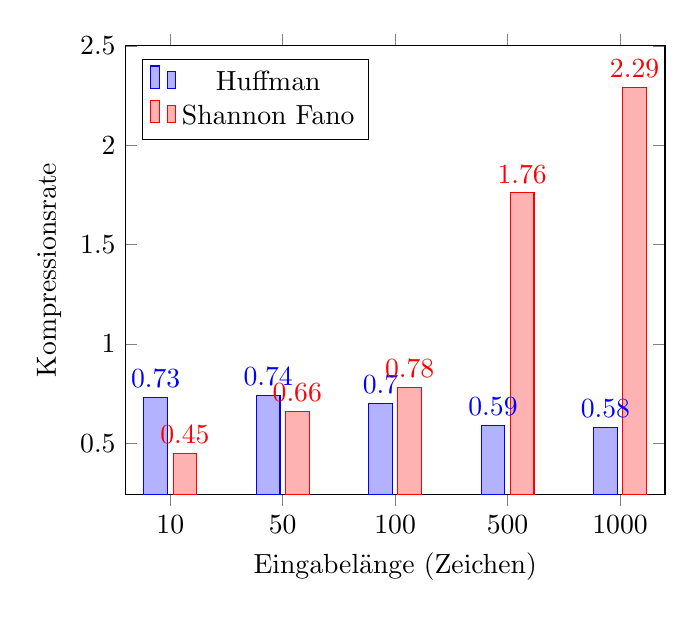
\begin{tikzpicture}
        \begin{axis}[
            legend pos=north west,
            bar width=0.3cm,
            ybar,
            ymax=2.5,
            symbolic x coords={10,50,100,500,1000},
            xtick=data,
            ylabel={Kompressionsrate},
            xlabel={Eingabelänge (Zeichen)},
            nodes near coords,
            nodes near coords align={vertical}]

        \addplot coordinates {(10,0.73) (50,0.74) (100,0.70) (500,0.59) (1000,0.58)};
        \addlegendentry{Huffman}
        \addplot coordinates {(10,0.45) (50,0.66) (100,0.78) (500,1.76) (1000,2.29)};
        \addlegendentry{Shannon Fano}

        \end{axis}
    \end{tikzpicture}
\end{center}
Die Tests spiegeln deutlich wieder, dass das Shannon-Fano Verfahren für Eingaben bis zu einer Länge von \textit{100} Zeichen im Allgemeinen eine bessere Kompressionsrate erbringt als die Huffman-Kodierung. Jedoch ändert sich dies drastisch bei größeren Zeichenketten.\\
Erklärt werden kann dies durch die rekursive Verteilung der Codes. Wenn die Eingabehäufigkeit aller Buchstaben relativ gleichverteilt ist, wird bei Shannon-Fano öfter und gleichmäßiger rekursiv aufgeteilt, was für jeden Code im Worst-Case $\mathcal{O}(\log(n))$ bedeutet. Anstatt sich die Häufigkeit zu Nutzen zu machen, wie es bei Huffman der Fall ist, wird (bei perfekter Aufteilung) ab einer Eingabe von \textit{256} Zeichen die Kompressionsrate höher als eine direkte Abbildung der Zeichen auf Bitrepräsentation ($\log_2(256)=8$). \cite{1819Vorlesung15a}
\subsection{Optimierung}
Die Korrektheit des Huffman Codes war von Anfang an gegeben, jedoch haben wir durch einige Optimierungen, die Zeit die unser Programm verbraucht hat, reduzieren können. Die benutzten Optimierungen werden im Folgenden untersucht.\\\\
Gemessen wurde die Hauptimplementierung ohne jegliche Ein-/Ausgabe auf \textit{10000} Durchläufen. Das \textit{print} Flag wurde nicht gesetzt, was alle Konsolenausgaben ausgeschaltet. Es wurden \textit{20} unterschiedliche \textit{Lorem ipsum}\cite{lorem_ipsum-generator_und_informationen} Texte in Rotation mit unterschiedlicher Eingabelänge bearbeitet. Trotz meist lateinischer Wörter stimmt die Verteilung der Häufigkeit des ausgewählten Text mit der der englischen als auch deutschen Sprache ausreichend überein, um aussagefähige Resultate zu erhalten.

\begin{center}
    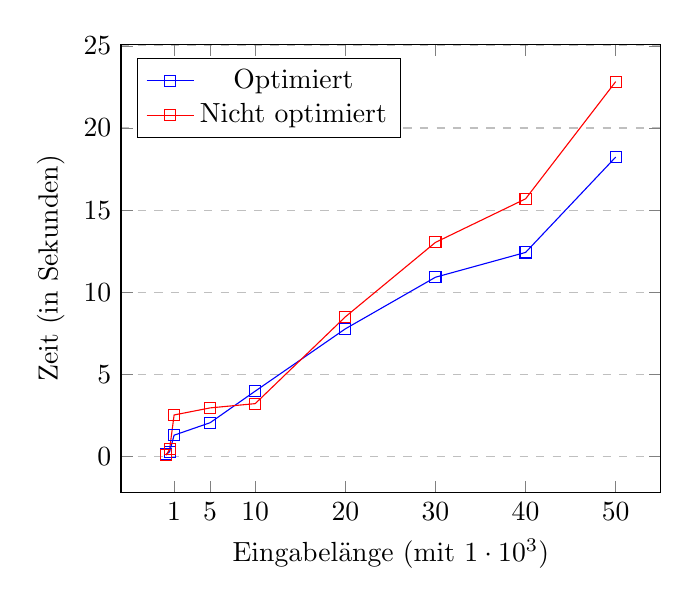
\begin{tikzpicture}
        \begin{axis}[
            xlabel={Eingabelänge (mit $1\cdot 10^3$)},
            ylabel={Zeit (in Sekunden)},
            xtick={1,5,10,20,30,40,50},
            legend pos=north west,
            ymajorgrids=true,
            grid style=dashed,
            ]

        \addplot[
            color=blue,
            mark=square,
            ]
            coordinates {
            (0.1,0.14)(0.5,0.30)(1,1.31)(5,2.07)(10,3.99)(20,7.78)(30,10.92)(40,12.43)(50,18.23)
            };

        \addplot[
            color=red,
            mark=square,
            ]
            coordinates {
            (0.1,0.09)(0.5,0.45)(1,2.54)(5,2.97)(10,3.23)(20,8.51)(30,13.04)(40,15.69)(50,22.82)
            };
            
        \legend{Optimiert, Nicht optimiert}
    
        \end{axis}
    \end{tikzpicture}
\end{center}
Wie zu erwarten klärt die Performanzmessungen auf, dass die optimierte Version eine bessere Laufzeit hervorbringt. Im Allgemeinen hat die Optimierung erst eine Auswirkung auf Eingaben mit Längen ab \textit{20000} Zeichen. Bei kleinen Eingaben macht es keinen großen Unterschied. Zudem scheint es, dass bei einem der Versuche eine unglückliche Textkombination dazu geführt hat, dass die unoptimierte Version eine bessere Laufzeit darstellt. Dies ist jedoch im Allgemeinen nicht zu erwarten.\\
Analysiert man den Quellcode des Programms, stellt sich heraus, dass besonders das Zählen der Textlängen zu erheblichen Verlangsamungen geführt haben. Dies wurde oft mit der \textit{strlen(const char *s)} Methode der \textit{string.h} C-Bibliothek provoziert. Eine Lösung hierfür ist nach dem Einlesen der Eingabe neben der Rückgabe der Daten auch die Länge zurückzugeben.\\
Außerdem wird die Häufigkeit zuerst in einem Array der Länge \textit{256} gezählt und erst im Anschluss werden die nicht leeren Häufigkeiten in einen Knoten transformiert. Dies sorgt für schnelleren Zugriff und es müssen nur maximal \textit{256} Knoten ohne weiteren Zugriff erstellt werden.\\
Zu guter Letzt wurde in der optimierten Version die Kodierung der Buchstaben zuerst in einem Dictionary gespeichert und anschließend jeder Buchstaben einzeln kodiert. In der alten Version hat man dies entlang des Baumes gemacht, was im schlimmsten Fall eine Laufzeit von $\mathcal{O}(log_2(n))$ bedeutet. Beim Aufbauen des Dictionaries muss dies allerdings nur einmal getan werden.\\
Leider ist eine Optimierung hinsichtlich der Erstellung des Baumes nur schwierig möglich, da immer die zwei kleinsten Häufigkeiten herausgenommen, zu einem Knoten verschmolzen und anschließend wieder hineingefügt werden. Daher ist es im Vorhinein unklar, wo sich der neu zu erstellende Knoten befinden wird. Dies sorgt dafür, dass eine Laufzeit unter $\mathcal{O}(n\cdot log2(n))$ nicht möglich ist.\\\\
\textit{
Die genannte Laufzeitanalyse wurde auf einem Apple MacBook Pro mit Silicon M1 Pro Chip, 16 GB Arbeitsspeicher und macOS Monterey 12.5.1 ausgeführt. Kompiliert wurde das Programm mit Apple clang version 14.0.0 (arm64-apple-darwin21.6.0) und der Option -O3. 
}

\section{Zusammenfassung und Ausblick}

Insgesamt ist der Huffman-Algorithmus aufgrund seiner Optimalität bei symbolbasierter Komprimierung immer noch sehr relevant, da er in den meisten Fällen sehr knapp an die durch die Entropie gegebene perfekte Komprimierung kommt.
Dennoch ist es möglich die Effizienz noch weiter zu erhöhen, indem man sich nicht nur auf symbolbasierte Algorithmen beschränkt.\\
Es wäre somit möglich, zum Beispiel bei von Menschen geschriebenen Fließtext, einen Huffman Baum für die einzelnen, durch Leerzeichen getrennte, Wörter zu erstellen. Dies könnte bei sehr großen Quelldateien, im Vergleich zum symbolbasierten Ansatz, effizienter sein.\\
Eine spezielle Anpassung auf das gespeicherte Format sollte ebenfalls zu Optimierungen führen. Man denke sich, zum Beispiel, \textit{PNG} für Bild- oder \textit{FLAC} für Audiodateien, da hier mehr Daten, als nur Buchstaben, abgespeichert werden müssen.\\
Zu der Implementierung kann man sagen, dass diese noch deutlich optimierbar ist. Zu einem ist das Verfahren mit den Min-Heap sehr anschaulich, aber dafür ineffizient, da es auch Lösungswege gibt, die dies in $\mathcal{O}(n)$ erreichen \cite{Leeuwen1976OnTC}, unter anderem auch in-place \cite{10.1007/3-540-60220-8_79}.
Das Speicherformat könnte ebenfalls weiter optimiert werden, indem man, anstatt diese menschenleslich zu strukturieren, direkt die Binärdaten reinschreibt. Zudem wäre es auch denkbar die Laufzeit, durch Parallelisierung und der Verwendung von mehreren Threads, zu reduzieren.\\
Zusammenfassend können wir sagen, dass wir durch das Projekt, zum optimierten Programmieren angeregt wurden und somit ein hoher Lerneffekt erlangt wurde.

\bibliographystyle{plain}
\bibliography{Ausarbeitung}{}

\end{document}
